\section{Реализация алгоритмов}

Все алгоритмы реализованы на языке \texttt{C++17}~\cite{Stroustrup}
в виде шаблонных функций в файле \texttt{sorting.cpp}
(см.~приложение~\ref{app:fullcode}). Использование шаблонов позволяет
сортировать любые типы данных, для которых определён оператор
\mintinline{cpp}{operator<}.

\subsection{Пузырьковая сортировка}

Функция \mintinline{cpp}{bubbleSort} принимает итераторы начала и
конца диапазона, аналогично функциям стандартной библиотеки. Флаг
\mintinline{cpp}{swapped} позволяет прервать цикл досрочно, если за
текущий проход не было ни одного обмена~--- это даёт сложность $O(n)$
на уже упорядоченных данных (см.~формулу~\ref{eq:bubble}).

\begin{minted}{cpp}
template <typename It>
void bubbleSort(It first, It last) {
    for (auto i = first; i != last; ++i) {
        bool swapped = false;
        for (auto j = first; j != std::prev(last, i - first + 1); ++j) {
            if (*std::next(j) < *j) {
                std::iter_swap(j, std::next(j));
                swapped = true;
            }
        }
        if (!swapped) break;
    }
}
\end{minted}

\subsection{Сортировка слиянием}

Функция \mintinline{cpp}{mergeSort} рекурсивно делит диапазон пополам
и вызывает вспомогательную функцию \mintinline{cpp}{merge} для слияния
двух упорядоченных половин. Временная буферная память выделяется
однократно и передаётся через параметр \mintinline{cpp}{buf}.

\begin{minted}{cpp}
template <typename It>
void merge(It first, It mid, It last, std::vector<typename It::value_type>& buf) {
    buf.clear();
    auto l = first, r = mid;
    while (l != mid && r != last)
        buf.push_back(*l < *r ? *l++ : *r++);
    buf.insert(buf.end(), l, mid);
    buf.insert(buf.end(), r, last);
    std::copy(buf.begin(), buf.end(), first);
}

template <typename It>
void mergeSort(It first, It last, std::vector<typename It::value_type>& buf) {
    if (std::distance(first, last) <= 1) return;
    auto mid = std::next(first, std::distance(first, last) / 2);
    mergeSort(first, mid, buf);
    mergeSort(mid, last, buf);
    merge(first, mid, last, buf);
}
\end{minted}

\subsection{Быстрая сортировка}

Функция \mintinline{cpp}{quickSort} использует в качестве опорного
элемента медиану из первого, среднего и последнего элементов
подмассива~--- это снижает вероятность вырожденного случая $O(n^2)$
(см.~формулу~\ref{eq:quicksort}).

\begin{minted}{cpp}
template <typename It>
It medianOfThree(It first, It last) {
    auto mid = std::next(first, std::distance(first, last) / 2);
    --last;
    if (*mid < *first) std::iter_swap(first, mid);
    if (*last < *first) std::iter_swap(first, last);
    if (*mid < *last)  std::iter_swap(mid, last);
    return last; // pivot at last
}

template <typename It>
void quickSort(It first, It last) {
    if (std::distance(first, last) <= 1) return;
    auto pivot = medianOfThree(first, last);
    auto p = std::partition(first, std::prev(last),
                            [&pivot](const auto& x){ return x < *pivot; });
    std::iter_swap(p, pivot);
    quickSort(first, p);
    quickSort(std::next(p), last);
}
\end{minted}

\begin{figure}[H]
    \centering
    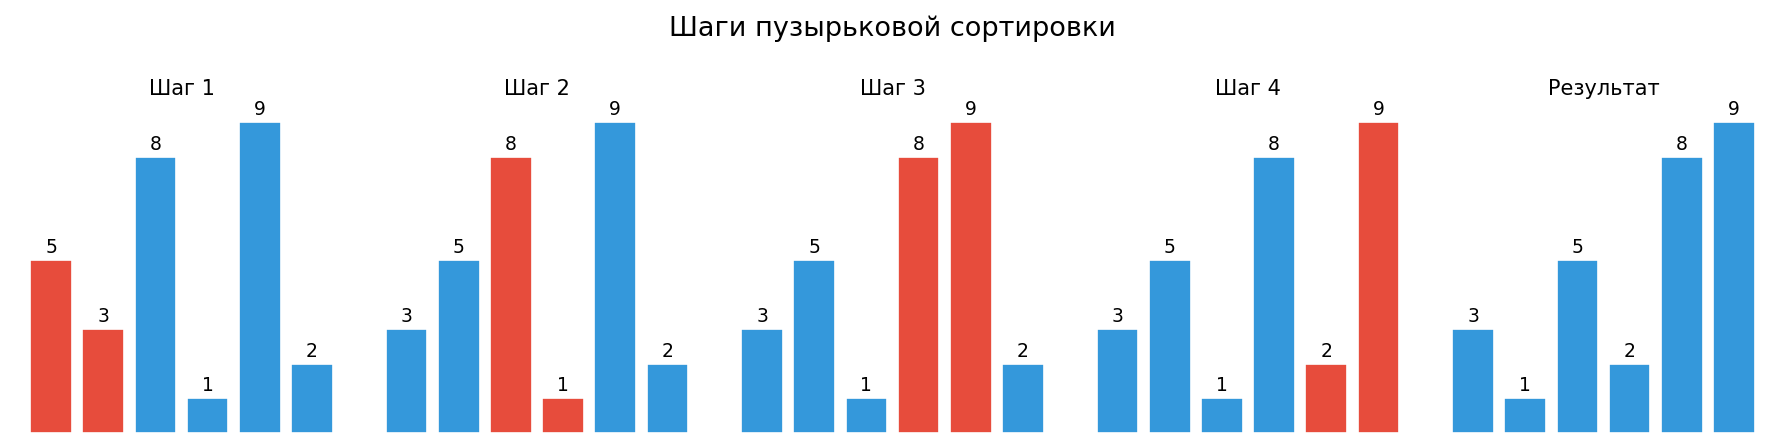
\includegraphics[width=0.85\textwidth]{images/bubble_steps.png}
    \caption{Шаги пузырьковой сортировки для массива из 6~элементов.
             Красным выделены сравниваемые элементы.}
    \label{fig:bubble_steps}
\end{figure}

На рисунке~\ref{fig:bubble_steps} показан пошаговый процесс работы
пузырьковой сортировки. На каждом шаге красным цветом выделена пара
элементов, которые сравниваются на данной итерации.
